\documentclass[a4j]{jarticle}
\usepackage{graphicx}
\usepackage{ascmac}
% \documentclass[11pt,a4paper]{ltjsarticle}
\usepackage{float}

\begin{document}

\title{計算機科学実験及演習4 DB \\ \bf 最終レポート}
% ↓ここに自分の氏名を記入
\author{上野山 遼音}
\date{提出日: \today} % コンパイル時の日付が自動で挿入される
\maketitle
\tableofcontents
\clearpage
\section{システム概要}
 今回作成したwebアプリケーション{\bf「KuBeat」} プロジェクトについて、概要をまとめる.現状と今後の完成目標を同時に記述する.
\subsection{システムの目的}
  本アプリケーションは、音楽ゲームアプリとSNSアプリを組み合わせたものである.
  音楽ゲームを通して、ユーザー同士の交流を促進することで、ユーザーの満足度を高める。
\section{モデル設計}
\subsection{実態関連図兼関係スキーマ}
\subsubsection{現状}
\begin{figure}[htbp]
  \centering
  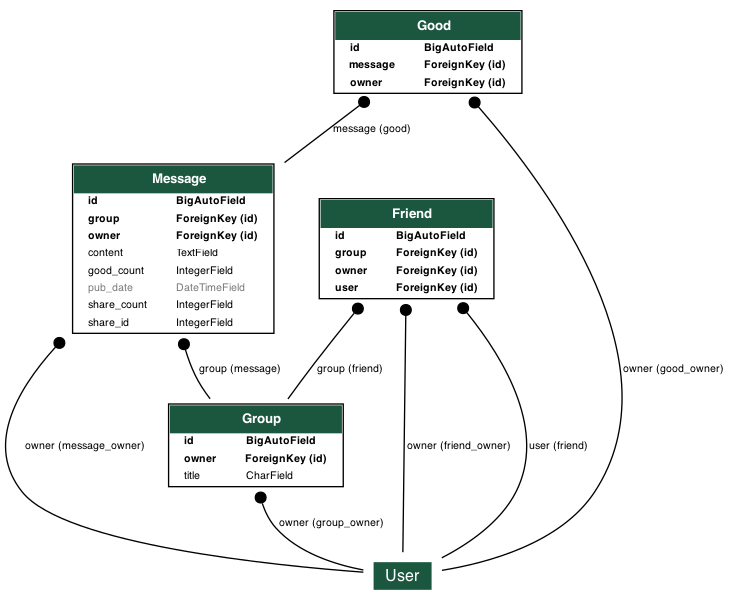
\includegraphics[width=0.8\textwidth,bb=0 0 800 600]{img/myer.png}
  \caption{ER図}
\end{figure}
\subsubsection{予定}
\begin{figure}[htbp]
  \centering
  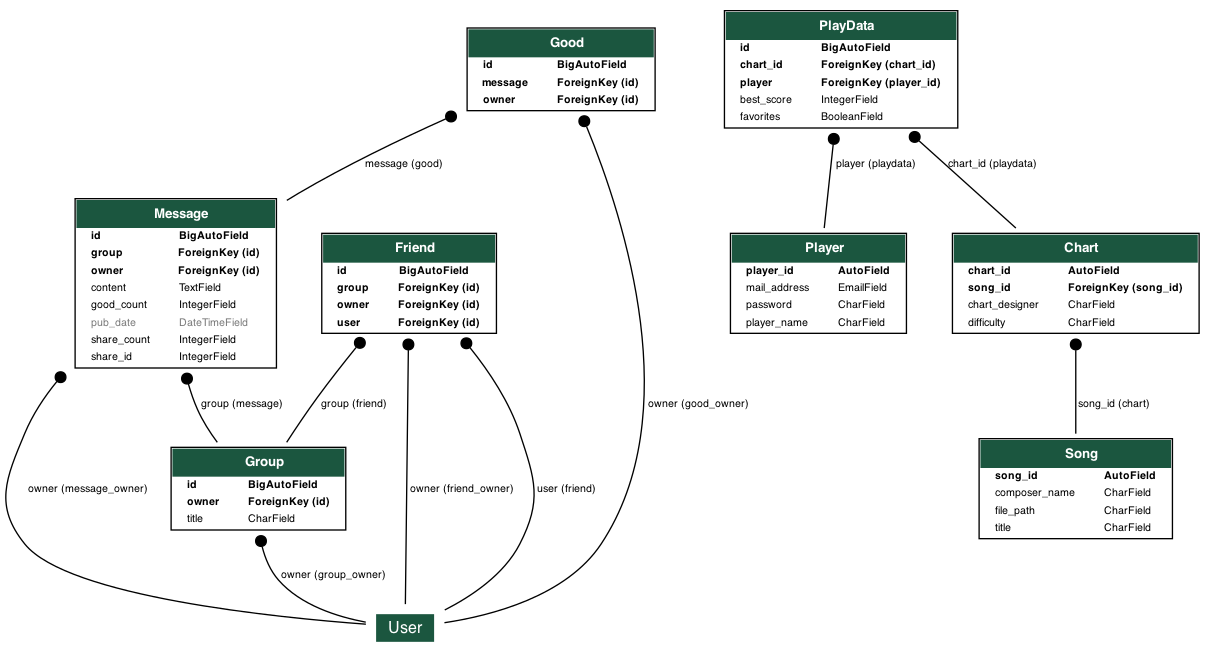
\includegraphics[width=0.8\textwidth,bb=0 0 800 600]{img/myer_goal.png}
  \caption{完成予定段階、フルで使われる予定でのER図}
\end{figure}
\clearpage
\section{画面構成}

\begin{figure}[htbp]
  \centering
  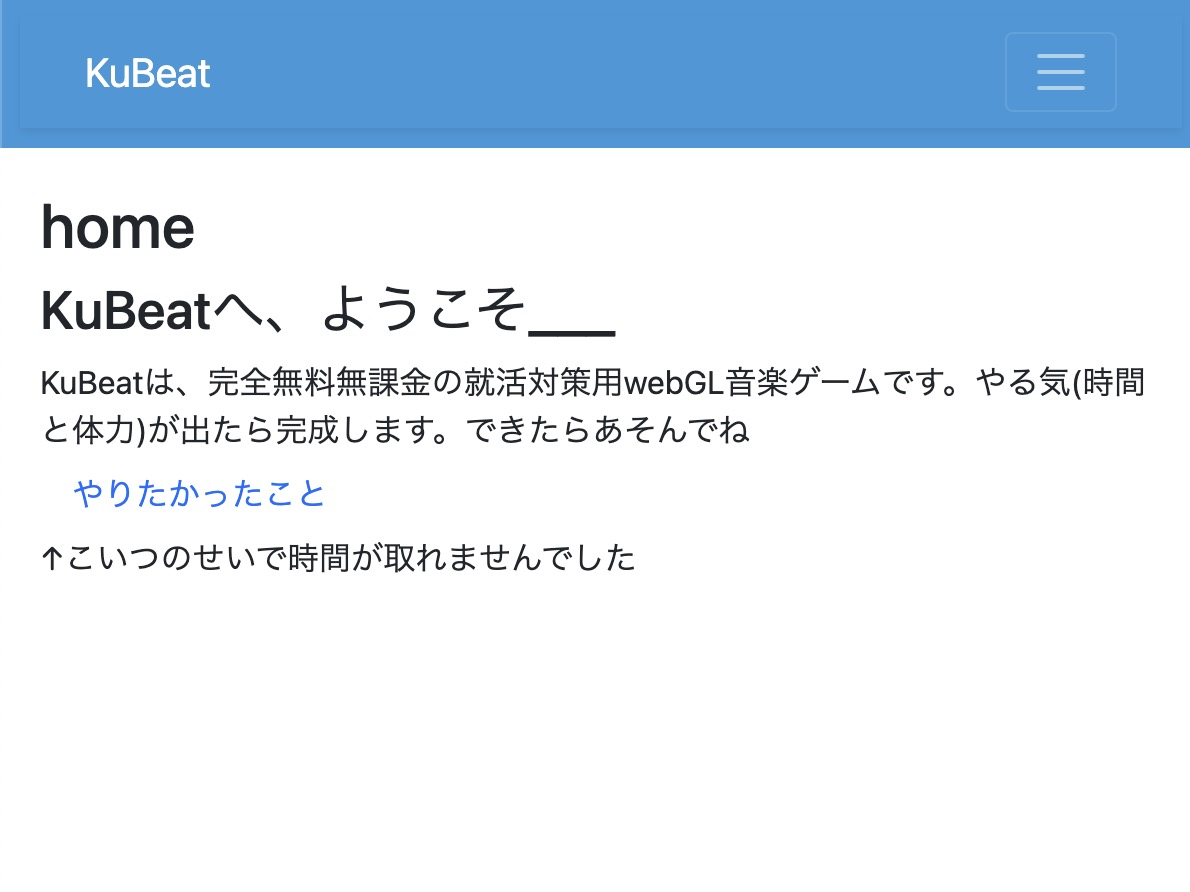
\includegraphics[width=0.8\textwidth,bb=0 0 800 600]{img/home.jpg}
  \caption{ホーム画面}
\end{figure}
% \begin{figure}[htbp]
%   \centering
%   \includegraphics[width=0.8\textwidth,bb=0 0 800 600]{img/.png}
%   \caption{ゲーム画面(のなりかけ)}
% \end{figure}
\begin{figure}[htbp]
  \centering
  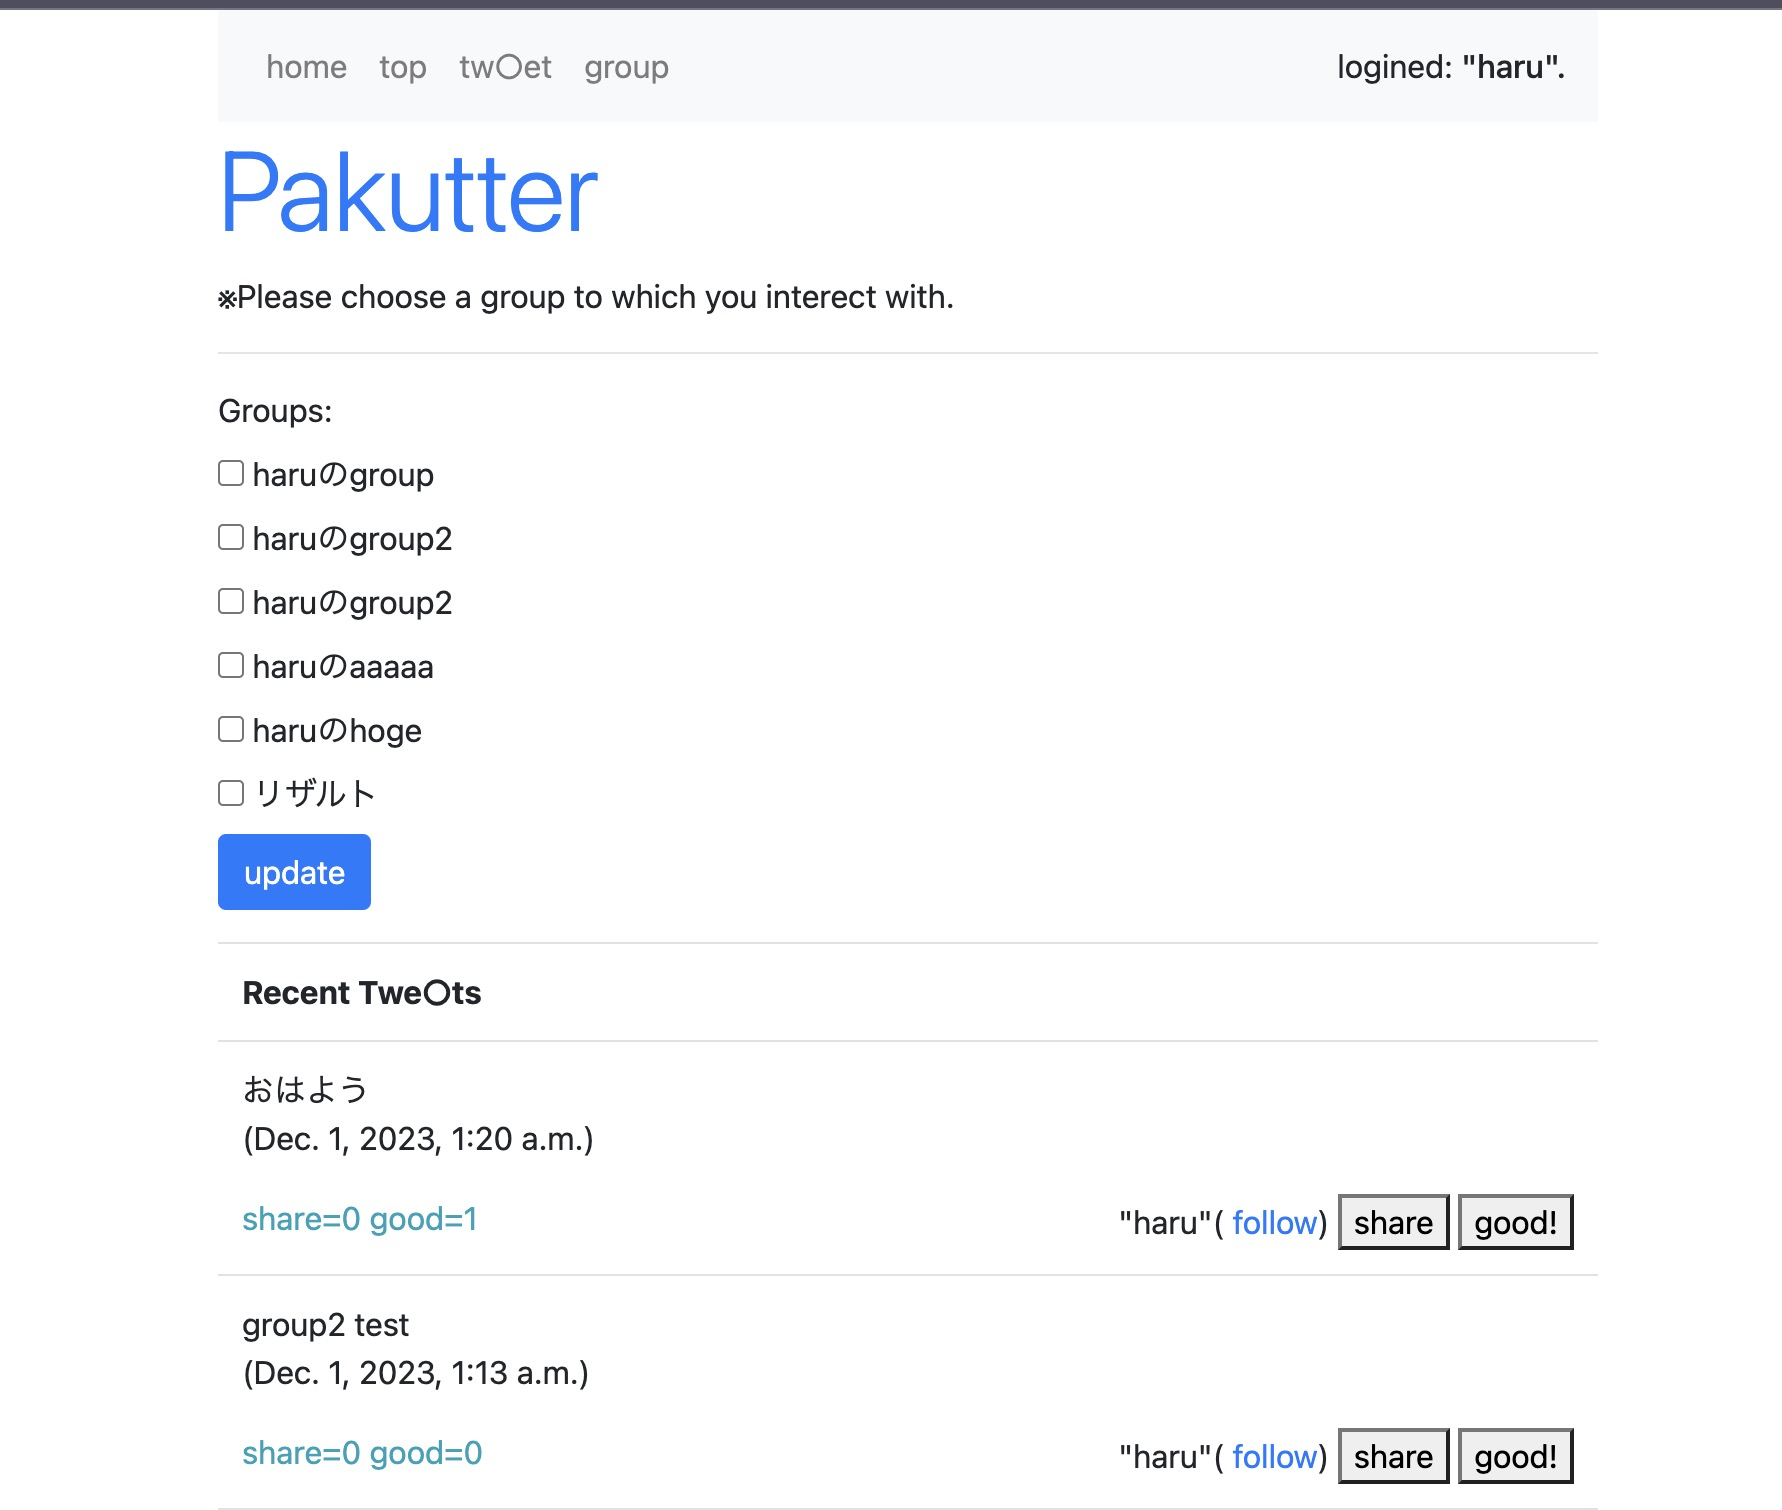
\includegraphics[width=0.8\textwidth,bb=0 0 800 600]{img/twitterhome.jpg}
  \caption{SNS機能ホーム画面}
\end{figure}
\section{機能一覧}
\subsection{現況}  
現状、以下の機能が完成している.
\subsubsection*{SNS機能: 命名 Pakutter}
\begin{itemize}
  \item ユーザー管理機能(管理者権限)
  \begin{itemize}
    \item ユーザー登録機能
    \item ユーザー情報編集機能
    \item ユーザー情報削除機能
    \item ユーザー情報一覧表示機能
  \end{itemize}
  \item 投稿機能(ユーザー権限)
  \item グループ作成機能(ユーザー権限)
  \item いいね、リツイート機能(ユーザー権限)
\end{itemize}
以下、各機能のインタフェースを示す。
\subsubsection{ユーザー管理機能}
djangoのadminサイトを利用して実装した.

\begin{figure}[htbp]
  \centering
  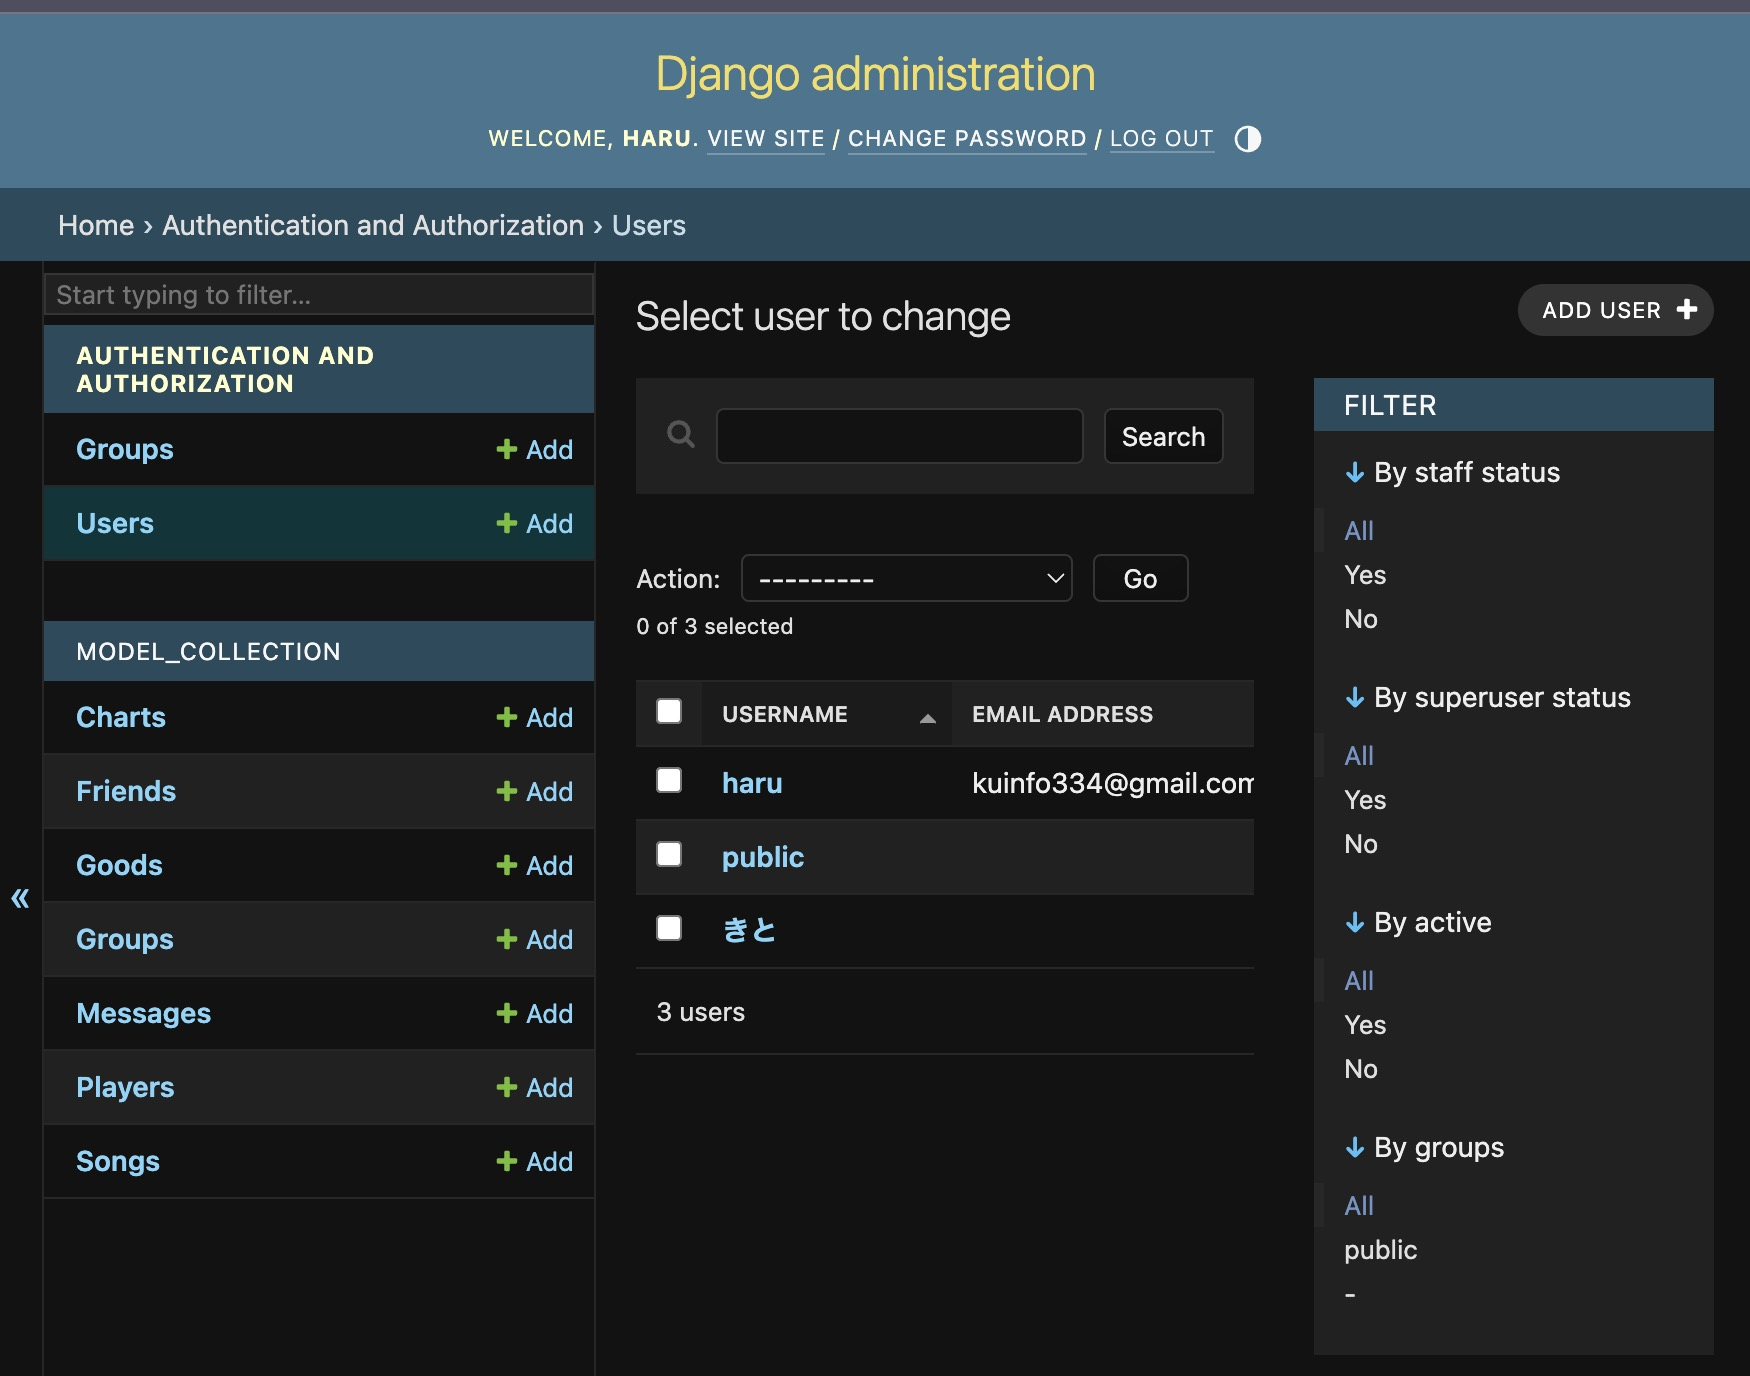
\includegraphics[width=0.8\textwidth,bb=0 0 800 600]{img/admin.jpg}
  \caption{ユーザー管理画面}
\end{figure}

\subsubsection{投稿機能}

\begin{figure}[htbp]
  \centering
  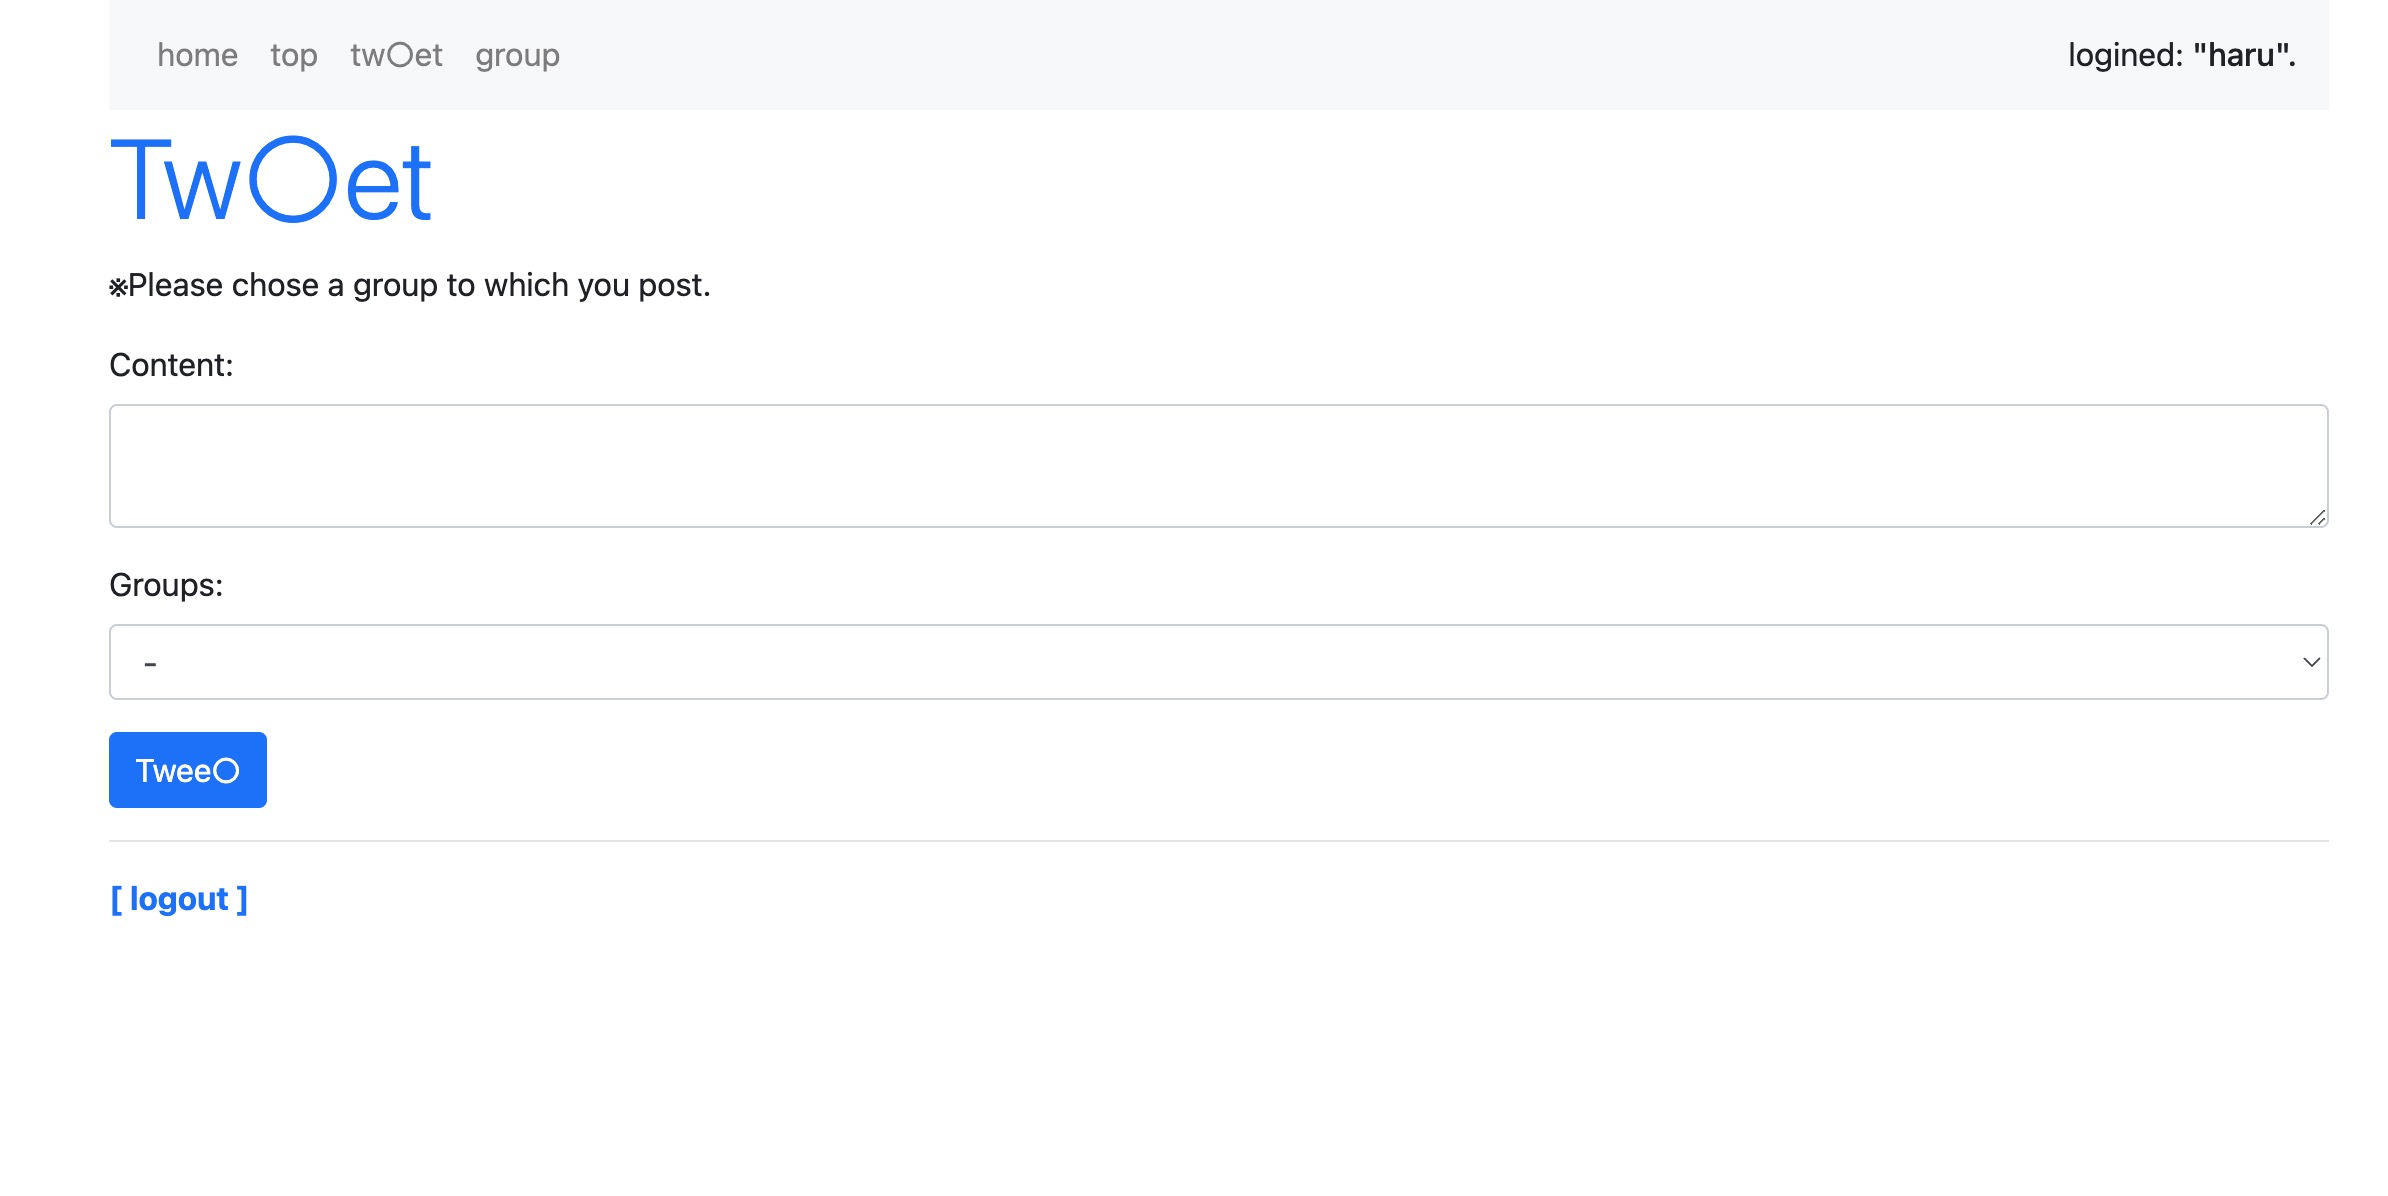
\includegraphics[width=0.8\textwidth,bb=0 0 800 600]{img/tweet.jpg}
  \caption{ポスト画面}
\end{figure}

\subsubsection{グループ作成機能}
\begin{figure}[htbp]
  \centering
  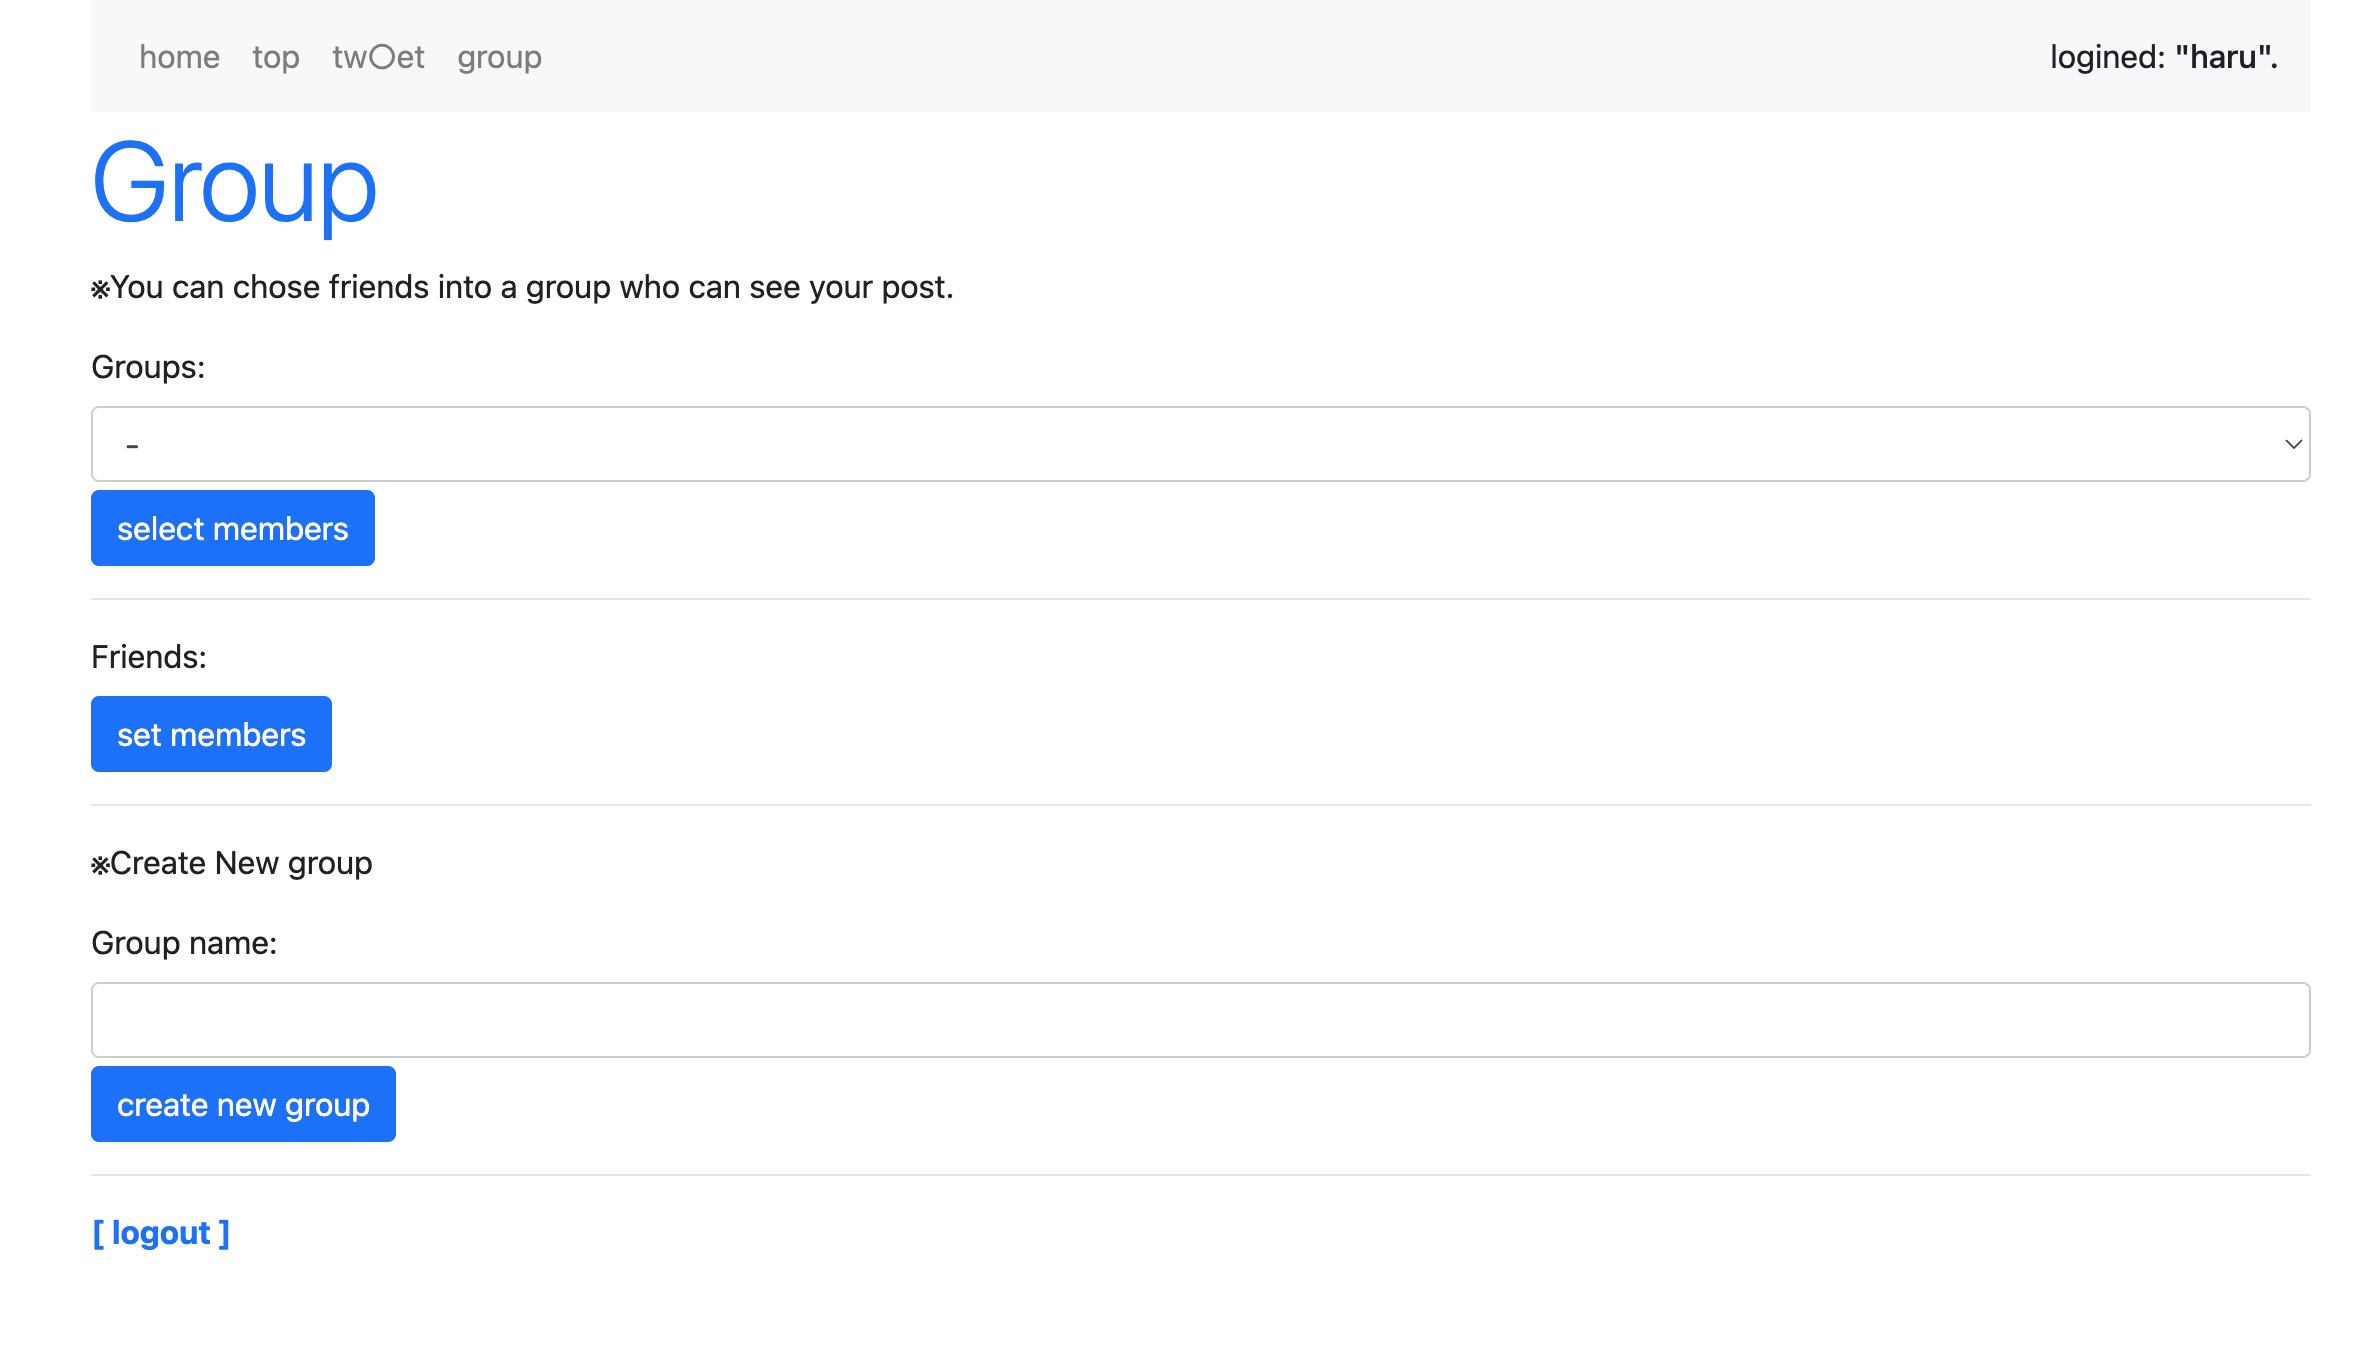
\includegraphics[width=0.8\textwidth,bb=0 0 800 600]{img/circle.jpg}
  \caption{グループ作成画面}
\end{figure}
\clearpage
\subsection{今後の完成目標}
現状完成している機能に加えて,以下の機能を実装することで、音楽ゲームアプリとして完成させる.
音楽ゲーム自体のコンセプトは、音響信号処理の実験で作成する予定のカラオケアプリを応用したものになる予定である。
\subsubsection*{音楽ゲーム機能: 命名 KuBeat}
\begin{itemize}
  \item スコアデータ(CR)管理機能
  \item 楽曲データ管理(CRUD)機能
  \item ランキング取得機能
  \item (そもそも音楽ゲームができるようにする)
\end{itemize}
\subsubsection*{SNS機能: 命名 Pakutter}
\begin{itemize}  
  \item リザルト投稿機能(ゲーム画面と連携)
  \item アカウント作成機能(ユーザー権限)
\end{itemize}

\section{工夫点}
ゲームエンジンのUnityと連携するために、djangoのAPIを利用し(ようとし)た.
\section{感想}
アプリの概念設計に関しては頑張れたと思う。しかしながら、実装に工数をあまり割けず、結果的に一晩で作り上げた状態になってしまい,今後の拡張に期待していただきたいという状況である。
デプロイはしておくので,ぜひ今後の成長をご覧いただきたい。
\end{document}